%%%%%%%%%%%%%%%%%%%%%%%%%%%%%%%%%%%%%%%%%%%%%%%%%%%%%%%%%%%%%%%%%%%%%%%%%%%%%%%%
\chapter{Обзор и сравнительный анализ существующих подходов}
%%%%%%%%%%%%%%%%%%%%%%%%%%%%%%%%%%%%%%%%%%%%%%%%%%%%%%%%%%%%%%%%%%%%%%%%%%%%%%%%
В данном разделе вводятся основные определения, связанные с предметной областью, приводятся различные классификации. Рассматриваются существующие подходы к обнаружению клонов и приводятся их основные характеристики.
%%%%%%%%%%%%%%%%%%%%%%%%%%%%%%%%%%%%%%%%%%%%%%%%%%%%%%%%%%%%%%%%%%%%%%%%%%%%%%%%
\section{Основные определения и классификация}

Для рассмотрения существующих подходов к обнаружению клонов, в первую очередь необходимо дать основные определения и классификации, связанные с предметной областью. 

\begin{itemize}
\item \textbf{Фрагмент кода} - часть исходного кода, необходимая для запуска программы. Такая часть может содержать в себе функцию или метод, блоки или последовательности операторов.
\item \textbf{Клон кода} - две и более части кода, которые аналогичны друг другу в соответствии с типами клонов.
\item \textbf{Клоновый класс} - максимальное множество фрагментов кода, в котором любые два фрагмента являются клонами.
\item \textbf{Кандидат в клоны} - пара фрагментов кода, которые были определены как клон.
\end{itemize}

С точки зрения идентичности дублированных фрагментов, клоны делятся на следующие типы:
\begin{itemize}
\item I: Полностью идентичные фрагменты программы без учета различий разметки и комментариев \cite{surveyroyandcordy} \cite{akhinitsykson}.
\item II: Клоны идентичные клонам первого типа, в которых также не учитваются различия идентификаторов, типов и литералов \cite{surveyroyandcordy} \cite{akhinitsykson}.
\item III: Клоны, идентичные клонам второго типа, в которых также не учитываются изменения, добавления и перемешивания операторов \cite{surveyroyandcordy} \cite{akhinitsykson}.
\item VI: Фрагменты программы, решающие схожую задачу, но реализованные различными способами (семантические клоны) \cite{surveyroyandcordy} \cite{akhinitsykson}.
\end{itemize}

При рассмотрении клонов с точки зрения их размера, выделяют следующие виды:
\begin{itemize}
\item С фиксированной гранулярностью: идентичные фрагменты кода фиксированного размера (методы классы и т.д.).
\item С производной гранулярностью: идентичные фрагменты произвольного размера
\end{itemize}


%%%%%%%%%%%%%%%%%%%%%%%%%%%%%%%%%%%%%%%%%%%%%%%%%%%%%%%%%%%%%%%%%%%%%%%%%%%%%%%%


\begin{figure}[htbp]
\centering
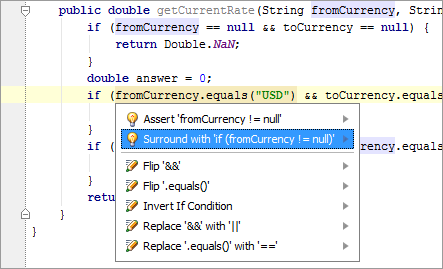
\includegraphics[width=\textwidth]{code_analysis_bugs.png}
\caption{Рекомендации по проведению исследований в рамках диссертации}%
\label{fig:how-to-do-research}
\end{figure}

\Blindtext

%%%%%%%%%%%%%%%%%%%%%%%%%%%%%%%%%%%%%%%%%%%%%%%%%%%%%%%%%%%%%%%%%%%%%%%%%%%%%%%%
\section{bar}
%%%%%%%%%%%%%%%%%%%%%%%%%%%%%%%%%%%%%%%%%%%%%%%%%%%%%%%%%%%%%%%%%%%%%%%%%%%%%%%%

\blindtext
It is of great importance that you use correct references in your dissertation.
Resent studies show that it can increase the chances of successful defense
by as much as 3,17 percent~\cite{russian, java-book, ANTLR}.

\Blindtext
